
\documentclass[12pt, a4paper, titlepage]{article}

\usepackage[spanish]{babel} % Soporte multilenguaje para LaTeX.
\usepackage{hyperref}
\usepackage[a4paper, top=2.5cm, bottom=2.5cm, left=2.5cm, right=2.5cm]{geometry}
\usepackage[utf8]{inputenc}
\usepackage{graphicx}
\usepackage{longtable}
\usepackage[usenames, dvipsnames]{color}
\usepackage{xcolor}
\usepackage[tikz]{bclogo}
\usepackage[framemethod=tikz]{mdframed}
\usepackage[many]{tcolorbox}
\usepackage{xcolor,listings}
\usepackage{amsmath}
\usepackage{fancyhdr}
\pagestyle{fancy}

\hypersetup{colorlinks, linkcolor=black, urlcolor=black}

\rhead{{\sl Arquitecturas y Plataformas Móviles}}

\begin{document}
	\begin{titlepage}
	
\includegraphics[width=15cm]{img/Simbolo_logo_UDC.png}
	% Lista de tamaños: \Huge, \huge, \LARGE, \Large, \large, \small, \footnotesize, \tiny
	\vspace{6cm}
		\begin{center}
			\Huge{\textbf{Arquitecturas y Plataformas Móviles}}

			\large{\textbf{Máster Universitario en Ingeniería Informática}}

		\end{center}
		\vspace{10cm}
		\begin{flushright}

			Alejandro Fortes Lopes

			Boris Caballero Lenza

			Javier Rochela Calvo

			Pablo Gómez Area

		\end{flushright}

		\vspace{1cm}
		\begin{flushright}
			A Coruña, \today
		\end{flushright}


	\end{titlepage}

	\clearpage

	\tableofcontents

	\clearpage

	\section{CEO}

	\clearpage

	\section{UX}

	\clearpage

    \section{Sensórica y geolocalización}
		En este apartado vamos a ver los elementos de sensórica utilizados en este proyecto, en este caso principalmente el uso de un sensor hardware que permite contar los pasos realizados.
    	\newline
    	\subsection{Introducción}
    	En versiones más antiguas de Android el conteo de pasos se realizaba leyendo directamente los datos del acelerómetro, que mide el cambio en la velocidad a lo largo de los tres ejes (X, Y, Z).
    	\newline
    	\begin{figure}[h!]
    		\begin{center}
    			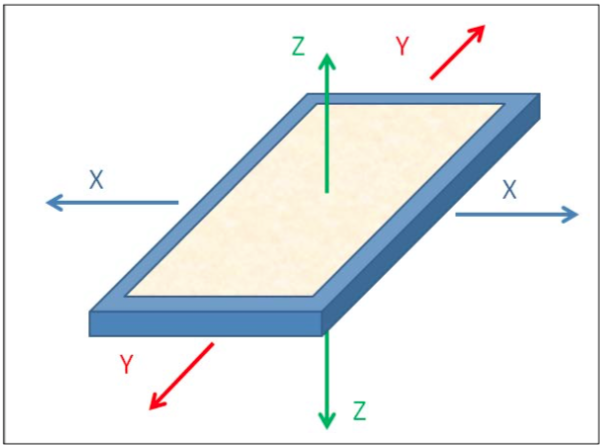
\includegraphics[scale=0.65]{img/ejes.png}
    			\caption{Ejes de coordenadas}
    		\end{center}
    	\end{figure}\\

    	Sin embargo, en este caso haremos uso de un sensor que nos proporcionan los dispositivos Android desde la versión 4.1, ya que consideramos que es una versión de Android relativamente antigua, y que abarcará a la inmensa mayoría de usuarios. Este es el sensor TYPE STEP COUNTER, ya que este activa un evento con cada paso detectado. También tendríamos la opción de usar TYPE STEP DETECTOR, pero los eventos TYPE STEP COUNTER se producen con una latencia mayor que aquellos que se generan desde TYPE STEP DETECTOR, eso se debe a que el algoritmo TYPE STEP COUNTER realiza un mayor procesamiento para eliminar los falsos positivos. Por lo tanto, TYPE STEP COUNTER puede ser más lento para generar los eventos, pero los resultados deben ser más precisos, con lo cual en este caso nos quedaremos con este último.

    	Una consideración muy importante a tener en cuenta, es que el TYPE STEP COUNTER solo se reinicia cuando se hace un reboot del dispositivo, así que deberemos tenerlo en cuenta para el correcto funcionamiento de la app, ya que debemos "reiniciarlo" virtualmente nosotros, para mostrar los pasos realizados desde la última apertura de la app.

    	\subsection{Metodos principales}
    	\begin{itemize}
    		\item \textbf{onCreate()}: En este método vamos a instanciar la clase SensorManager para poder obtener información y tener acceso a los sensores del sistema\newline\\

    		\begin{figure}[h!]
    			\begin{center}
    				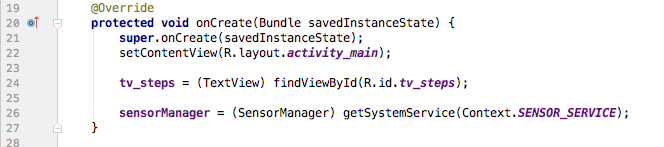
\includegraphics[scale=0.55]{img/onCreate.png}
    				\caption{Método onCreate()}
    			\end{center}
    		\end{figure}
    		\item \textbf{onResume()}: Si nuestra aplicación por alguna razón pasa por el método onPause, dejará de obtener los datos, por lo que si entraramos de nuevo no tendríamos respuesta, es por ello que hay que sustituir este método para volver a extraer la información.\newline\\
    		Análogamente al metodo onCreate, volvemos a hacer uso de la clase SensorManager para recoger los sensores TYPE STEP COUNTER, y además en el caso de que se haya encontrado, registramos un listener el cuál acepta como parámetros el Context de nuestra Activity, el sensor que queremos registrar, si es que se ha encontrado, y una constante que recaudará los datos a una velocidad determinada. En este caso hemos escogido como constante de velocidad SENSOR DELAY IU. \newline\\

    		En el caso de no encontrar el sensor que estamos utilizando, se lanzará un Toast de aviso.
    		\begin{figure}[h!]
    			\begin{center}
    				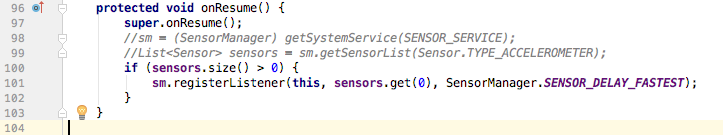
\includegraphics[scale=0.55]{img/onResume.png}
    				\caption{Método onResume()}
    			\end{center}
    		\end{figure}\\
    		\item \textbf{onPause()}: En este método tendríamos dos opciones, o bien protegernos de un gasto desmesurado de la batería, que sería provocado al tener que salir de la aplicación. Para evitar esto dejariamos de registrar el listener en el SensorManager cuando la actividad entrase en estado de pausa y evitar así que siguiera extrayendo datos del sensor.\newline\\
    		Sin embargo hemos optado por no hacerlo, ya que consideramos que en el uso de nuestra aplicación no tendría mucho sentido dejar de registrar los pasos aún con la aplicación en estado de pausa. A pesar de esto, si quisieramos cambiar dicha configuración sería tan sencillo como descomentar la linea 46 de la siguiente imagen.
    		\begin{figure}[h!]
    			\begin{center}
    				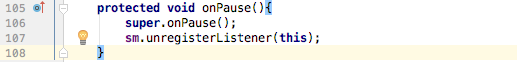
\includegraphics[scale=0.55]{img/onPause.png}
    				\caption{Método onPause()}
    			\end{center}
    		\end{figure}\\
    		\item \textbf{onStop()}: Al contrario de lo que hemos hecho en el método onPause(), en este método si quitamos el registro del listener en el SensorManager antes de cerrar la actividad, ya que una vez cerrada no tendría sentido seguir extrayendo datos del sensor, y nos crearía un serio problema de consumo de batería.\newline\\
    		\begin{figure}[h!]
    			\begin{center}
    				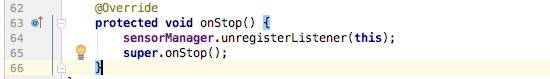
\includegraphics[scale=0.55]{img/onStop.png}
    				\caption{Método onStop()}
    			\end{center}
    		\end{figure}\\
    		\item \textbf{onSensorChanged()}: Este método se ejecutará siempre y cuando cambie algun valor del sensor. En este caso, primero comprobamos si la app está ejecutandose, y si es el caso se muestra el valor en pantalla.
    		\begin{figure}[h!]
    			\begin{center}
    				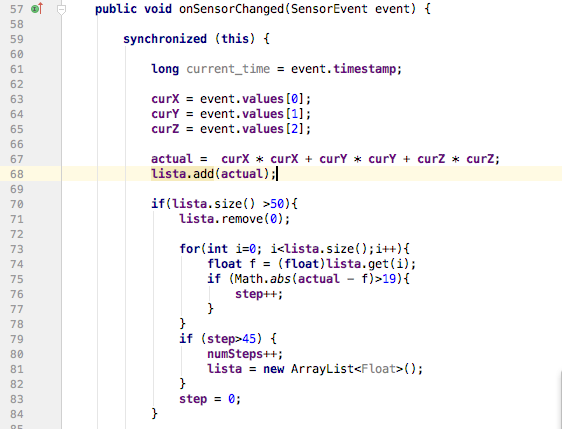
\includegraphics[scale=0.55]{img/onSensorChanged.png}
    				\caption{Método onSensorChanged()}
    			\end{center}
    		\end{figure}\\
    		\item \textbf{onAccuracyChanged}: este sería el método donde deberíamos implementar las acciones a realizar si la precisión del sensor cambia, en este caso no realizaremos ninguna ya que no lo consideramos necesario, pero es igualmente necesario declararlo.
    	\end{itemize}

    	\subsection{Vistas  dentro de la app}

        	En la siguiente imagen vemos la vista del contador de pasos de la app.
        	\begin{figure}[h!]
        		\begin{center}
        			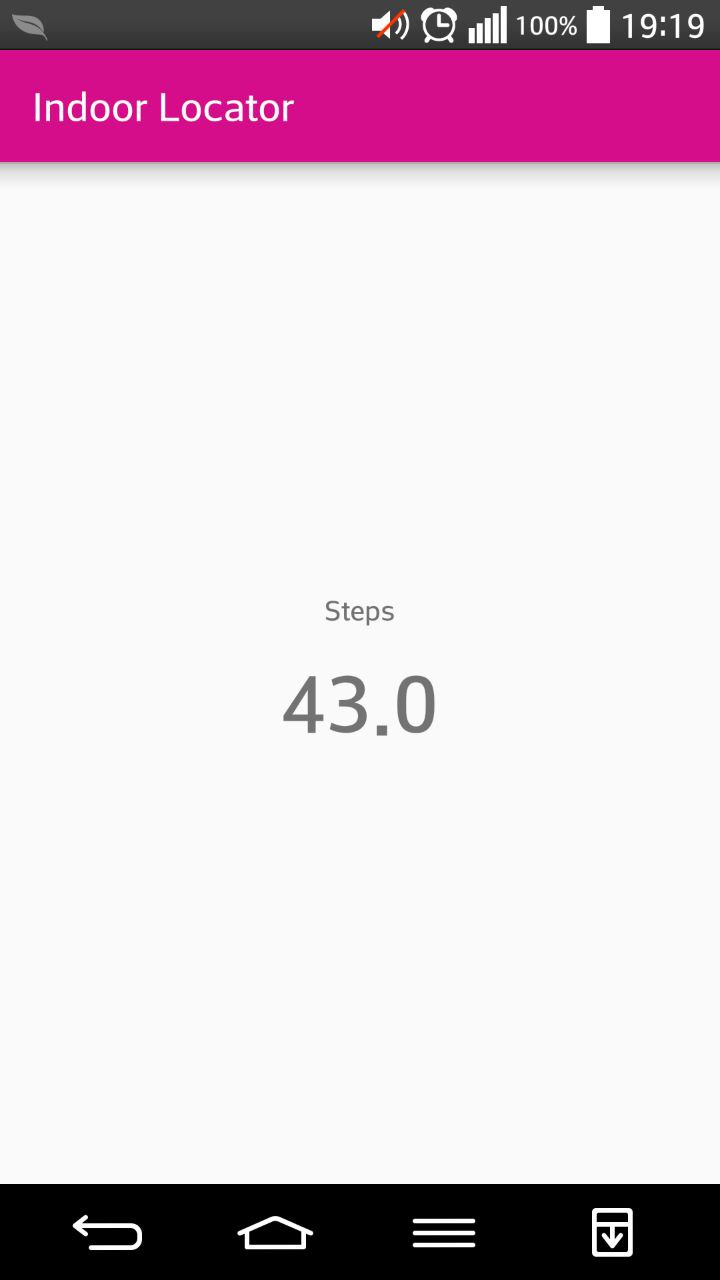
\includegraphics[scale=0.25]{img/steps.png}
        			\caption{Vista de los pasos en la app}
        		\end{center}
        	\end{figure}

        	En el caso poco probable de que la versión de Android sea anterior a la 4.1, el sensor no será detectado.

        		\begin{figure}[h!]
        			\begin{center}
        				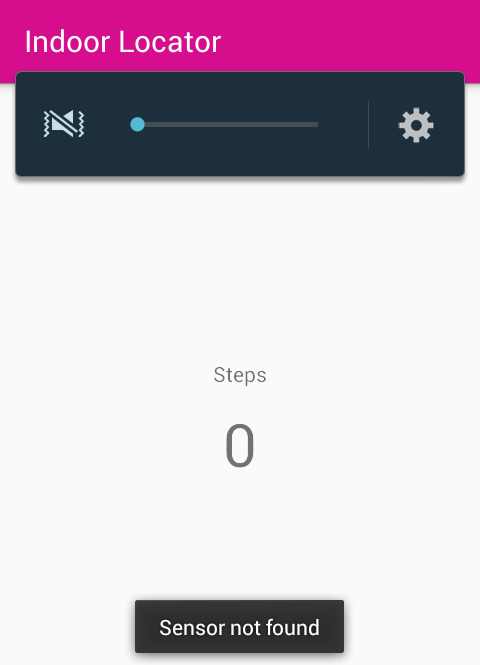
\includegraphics[scale=0.45]{img/notFound.png}
        				\caption{Sensor no encontrado}
        			\end{center}
        		\end{figure}
	\clearpage

	\section{APIs}
	En este apartado vamos a ver el control de acceso de la aplicación, la obtención de información sobre los profesores y los despachos, y la persistencia de esta información.
	
	\subsection{Acceso a la aplicación}
		\begin{figure}[h!]
		\begin{center}
			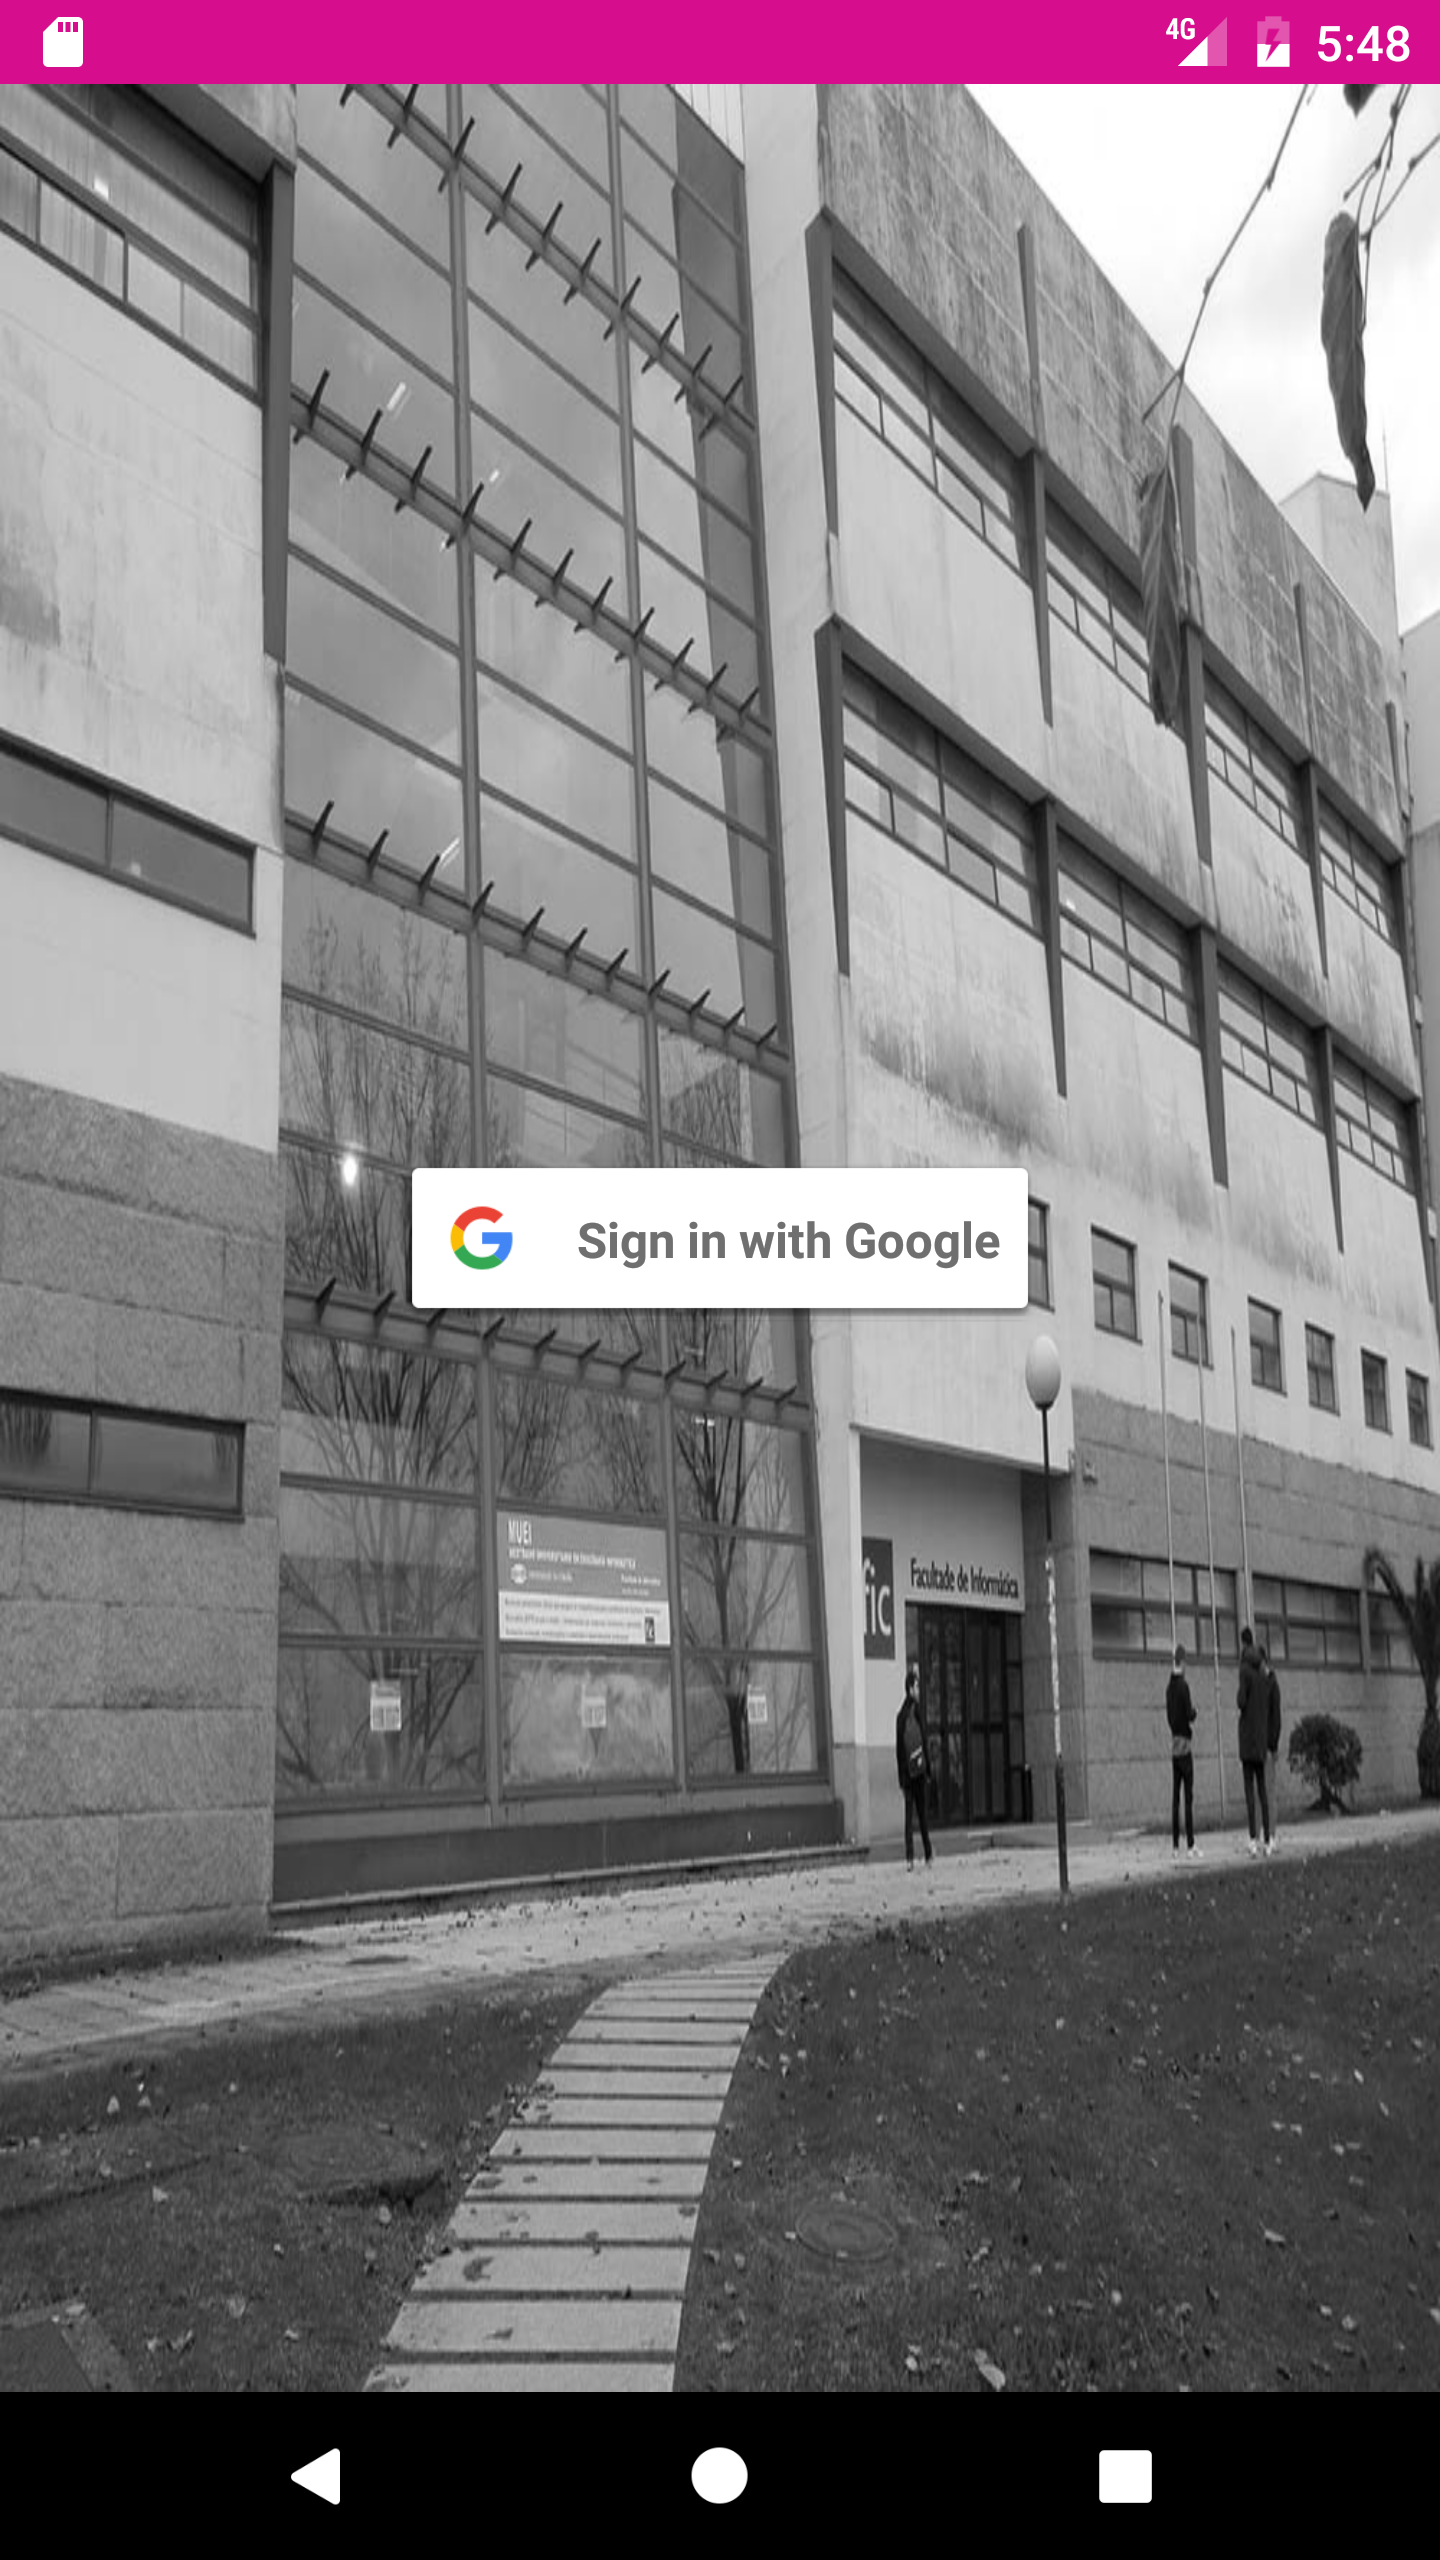
\includegraphics[scale=0.15]{img/login.png}
			\caption{Login de la aplicación}
		\end{center}
	\end{figure}
	
	Como se puede ver en la imagen superior hemos optado por utilizar el login de Google, para dotar a nuestra aplicación de autenticación. El flujo para la autenticación es el siguiente:
	\begin{enumerate}
		\item Primero se intenta acceder sin que el usuario tenga que realizar ninguna acción.
		\item Si es posible, el usuario ya autenticado accede a la aplicación
		\item En caso contrario, se le da la opción al usuario de acceder de forma manual, bien utilizando una cuenta de su dispositivo, o bien introduciendo una nueva dirección de correo y una clave. La api de Google también da la opción de crear una nueva cuenta.
		\item Una vez autenticado el usuario accede a la aplicación.
	\end{enumerate}
	\subsection{Obtención de información}
	Para este punto hemos optado por crear nuestro propio servidor web REST dado que no existe un servicio web que nos permita disponer de esta información. Este servidor tiene implementados cinco métodos que permiten acceder a la información de diferentes profesores en formato JSON. Estos métodos son: 
	\begin{itemize}
		\item GET <<server>>/api/rooms/: permite obtener una lista de las salas de la planta.
		\item GET <<server>>/api/rooms/\{id\}: permite obtener la información de una sala en concreto.
		\item GET <<server>>/api/teachers/: permite obtener una lista de todos los profesores.
		\item GET <<server>>/api/teachers/\{name\}:  permite obtener la información de un profesor en concreto.
		\item GET <<server>>/api/all/:  permite obtener toda la información disponible.
	\end{itemize}
	Estos métodos son invocados desde la aplicación mediante \textit{AsyncTasks} con excepción de la última que se ejecuta thread ya que suponemos que en una aplicación un poco mas grande excedería la duración recomendada para una \textit{AsyncTask}.\\
	La clase \textit{TeachersTask} es la encargada de hacer estas peticiones, y es utilizada desde las clases \textit{TeacherFragment} y \textit{OthersFragment} siempre y cuando el flag \textit{teachersLoaded} (del que se hablará en el siguiente apartado) tenga valor negativo.
	
	\subsection{Persistencia}
	La aplicación permite sincronizar los datos obtenidos mediante el servicio web REST mencionado en el apartado anterior y almacenarlos en una base de datos para evitar futuras llamadas al servicio y reducir el consumo de datos de la aplicación.
	Esta opción esta disponible en el menú superior, bajo el nombre de Sincronizar. Esta opción solamente estará disponible si tenemos una conexión WIFI activa.\\
	
	\begin{figure}[h!]
		\begin{center}
			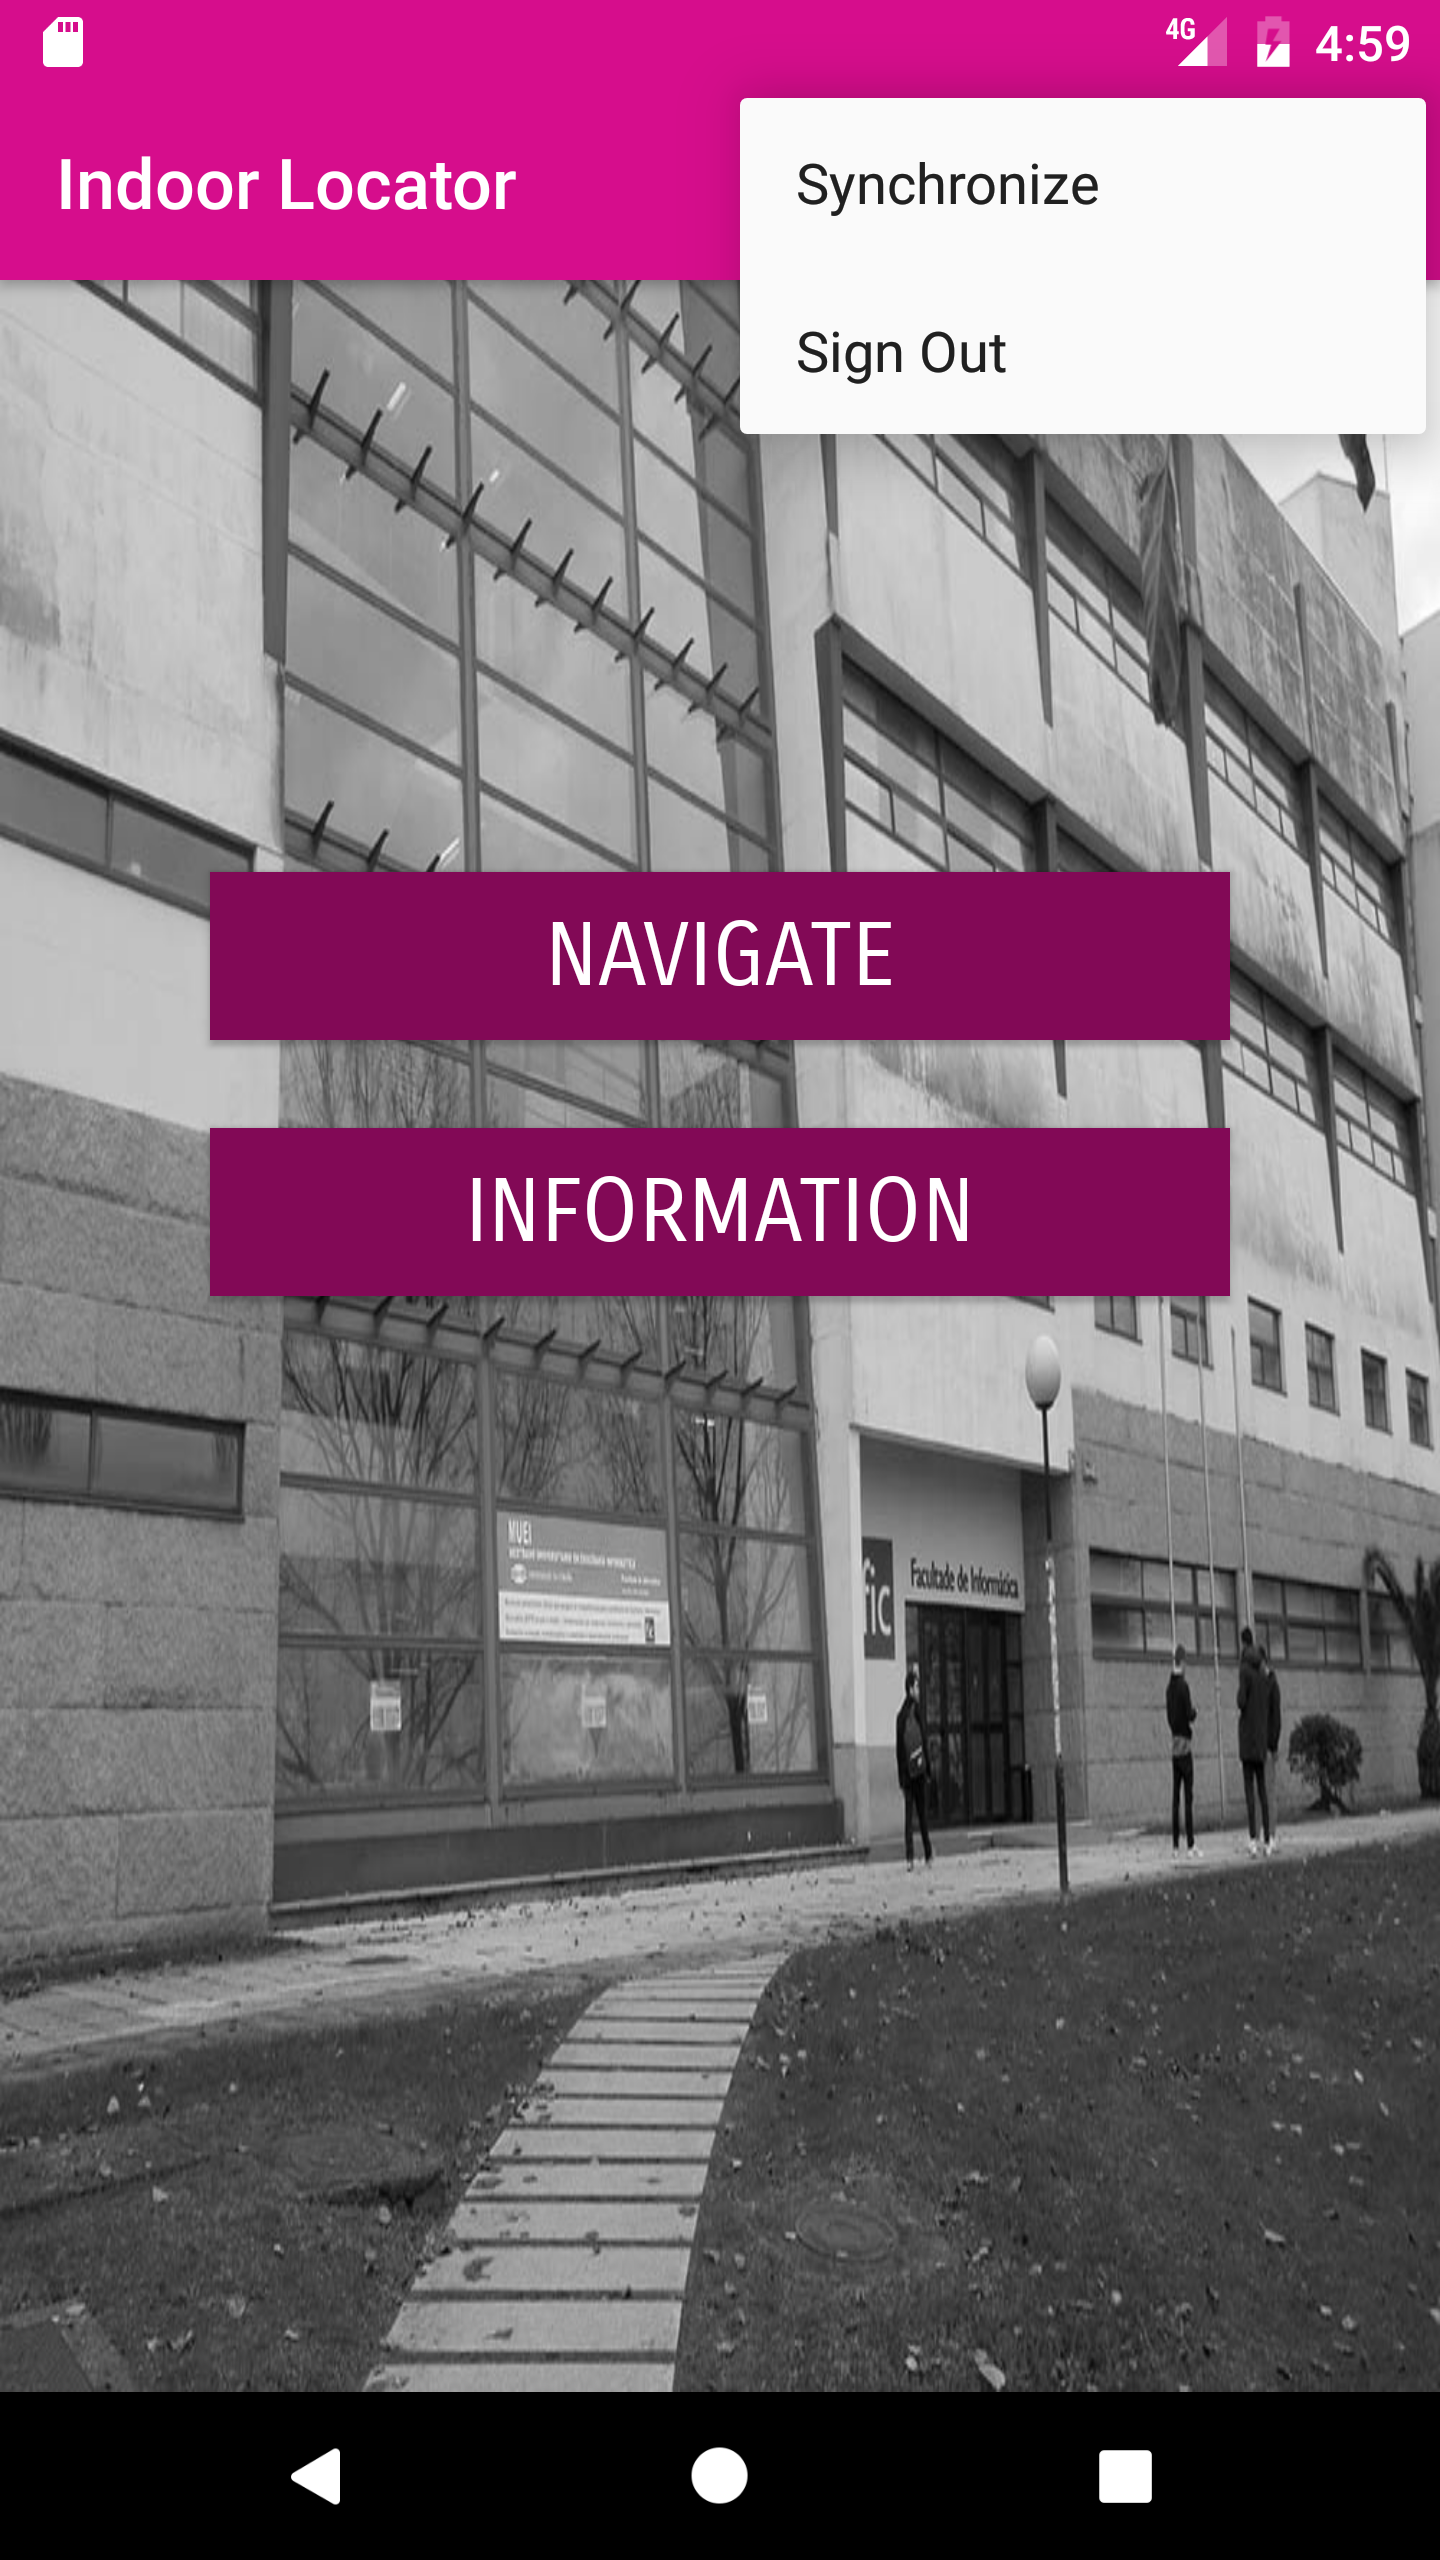
\includegraphics[scale=0.15]{img/menu_sincronizar.png}
			\caption{Imagen de la opción de Sincronizar}
		\end{center}
	\end{figure}
	
	Al pulsar sobre esta opción se iniciará el proceso siguiente:
	\begin{enumerate}
		\item Se lanza en un nuevo thread, una petición al servicio web REST para obtener todos los datos.
		\item Se procesa la respuesta de la petición y se convierte el JSON obtenido en objetos de tipo \textit{Teacher}.
		\item Dependiendo del valor de la variable \textit{teachersLoaded} que indica si esta operación se ha llevado a cabo con anterioridad, se elimina el contenido actual de la base de datos.
		\item A continuación se insertan en la base de datos la nueva información
		\item Por último se modifica el valor de la variable \textit{teachersLoaded} y se guarda en el archivo de preferencias compartidas de la aplicación.
	\end{enumerate}	
	
	A partir de este momento ya no se necesitará mas el servidor REST, dado que, en su lugar se harán las peticiones correspondientes a la base de datos.\\
	En está base de datos quedará almacenada una tabla \textit{Teachers} que tendrá los siguientes atributos.
	\begin{itemize}
		\item \textbf{Id}: Identificador único de usuario. (generado automáticamente por la base de datos)
		\item \textbf{name}: Nombre. 
		\item \textbf{department}: Departamento.
		\item  \textbf{job}: Puesto de trabajo.
		\item \textbf{office}: Despacho del profesor.
		\item \textbf{extension}: Extensión telefónica.
		\item \textbf{email}: Dirección de correo electrónico.
	\end{itemize}
	
	\clearpage

	\section{Realidad aumentada}



\end{document}









